\section{Part 2}
\subsection*{Categorical Density Estimation}
Proportion of times different categories appear, 
ordering of variables in CDF do not matter\\
\[\Pr(x\mid\Theta)=\theta_1^{I{[x=1]}}\dots\theta_k^{I{[x=k]}},\sum_c \theta_c=1\]
$\theta_C$ parameterization and unnormalized prob $\tilde{\theta}_C$\\
\[\theta_{c,MLE}=\frac{n_c}{n}\]
\subsection*{Dirichlet Distribution}
Prob Dsb over discrete prob dsbs, used as prior for Categorical
\[\Pr(\Theta\mid\alpha)\propto \prod_c \theta_c^{\alpha_c-1}\]
MAP w Dirichlet generalizes Laplace smoothing
\subsection*{Categorical Distribution Inference}
\begin{enumerate}
    \item Union, $\Pr(x=2\cup x=3\mid\Theta)$ or CDF
    \item Decoding, $\argmax_c \theta_c$
    \item Dataset Prob, $\Pr(X\mid\Theta)$
    \item Sampling
\end{enumerate}
\subsection*{Monte Carlo}
Approx expectations of random fns.\\
Generate samples, ave fn value applied to each sample.\\
Use Indicator function to approx prob of event
\subsection*{Conjugate Priors}
Given likelihood, prior leads to posterior of same family\\
\[x\sim D(\theta), \theta\sim P(\lambda) \Rightarrow \theta\mid x \sim P(\lambda')\]
\begin{center}
\begin{tabular}{||c c||} 
    \hline
    Likelihood & Prior \\ [0.5ex] 
    \hline\hline
    Bernoulli/Binomial & Beta  \\ 
    \hline
    Poisson/Exponential & Gamma\\
    \hline
    Categorical/Multinomial & Dirichlet \\
    \hline
    Normal (known var) & Normal \\
    \hline
    Normal (known mean) & Inverse Gamma\\
    \hline
    Multivariate Normal (known mean) & Inverse-Wishart\\ [1ex] 
    \hline
\end{tabular}
\end{center}
\subsection*{Conditional Independence Assumptions}
Hidden data-generating process $\mathcal{D}$
\begin{enumerate}
    \item IID data
    \[x^i\perp x^j \mid \mathcal{D}\]
    \item Independence of data given parameters
    \[x^i\perp x^j \mid \theta,\mathcal{D}\]
    \item Data independent of hyper-params given param
    \[X\perp \alpha,\beta \mid \theta\]
    \item Discriminative models assume params ind. features
    \[w\perp X\]
\end{enumerate}
\subsection*{Bayesian Probabilities}
\begin{enumerate}
    \item Prior ("regularizer")
    \[\Pr(\theta\mid\alpha)\]
    \item Likelihood
    \[\Pr(X\mid\theta)\]
    \item Posterior
    \[\Pr(\theta\mid X,\alpha)\]
    \item Marginal Likelihood
    \[\Pr(X\mid\alpha)\]
    \item Posterior Predictive
    \[\Pr(\tilde{X}\mid X,\alpha)\]
\end{enumerate}
\subsection*{Learning Principles}
\begin{enumerate}
    \item MLE - Maximize prob of data given params (likelihood)
    \[\hat{\theta}\in\argmax_{\theta}\{\Pr(X\mid\theta)\}\]
    \[\hat{x}\in\argmax_x \{\Pr(x\mid\theta)\}\]
    \item MAP - Maximize prob of paras given data (posterior)
    \[\hat{\theta}\in\argmax_{\theta}\{\Pr(\theta\mid X,\alpha)\}\]
    \[\hat{x}\in\argmax_x \{\Pr(x\mid\theta)\}\]
    \item Bayesian ("no learning")
    \[\hat{x}\in\argmax_x \{\Pr(x\mid X,\alpha)\}\]
    \[\equiv \argmax_x\{\int\Pr(\theta\mid X,\alpha)\Pr(x\mid\theta)d\theta\}\]
    \item Empirical Bayes - Type II MLE
    \[\hat{\alpha}\in\argmax_{\alpha}\{\Pr(X\mid\alpha)\}\]
    \[\hat{x}\in\argmax_x\{\Pr(x\mid X,\tilde{\alpha})\}\]
\end{enumerate}
\subsection*{Bayesian Learning}
Sum/integrate over all params, combine likelihood w prior\\
Posterior predictive, possibly cost fn for Bayesian decision theory\\
Strong protection against overfitting - regularizing and averaging
\subsection*{Empirical Bayes}
Optimize hyper-params using marginal likelihood\\
Can optimize large no. of hyper-params w/o validation set\\
Type II MLE / Evidence Maximization
\subsection*{Hierarchical Bayes}
Prior on prior, to model non-IID grouped data
\subsection*{Multi-Class Classification}
\begin{itemize}
    \item Supervised learning w categorical labels
    \item Tabular Probabilities - exp no. of params
    \item Bayesian Decision Theory - given cost fn, optimize expected cost under posterior predictive
    \item Categorical generalization of sigmoid is softmax\\
    Softmax fn converts k real numbers into probability
    \[f_c(Z)=\frac{\exp z_c}{\sum_{c'}\exp z_{c'}}\]
    \item Multi-Class Neural Networks: Softmax on last layer
\end{itemize}
\subsection*{What have we learned?}
Layers doing something sensible\\
ML models easily fooled
\begin{itemize}
    \item Unpredictable performance on 'out of distribution' images
    \item Adversarial examples lead to incorrect predictions
    \item Do not understand context and obvious confounding factors
\end{itemize}
Harmful biases
\subsection*{Recurrent Neural Networks (RNNs)}
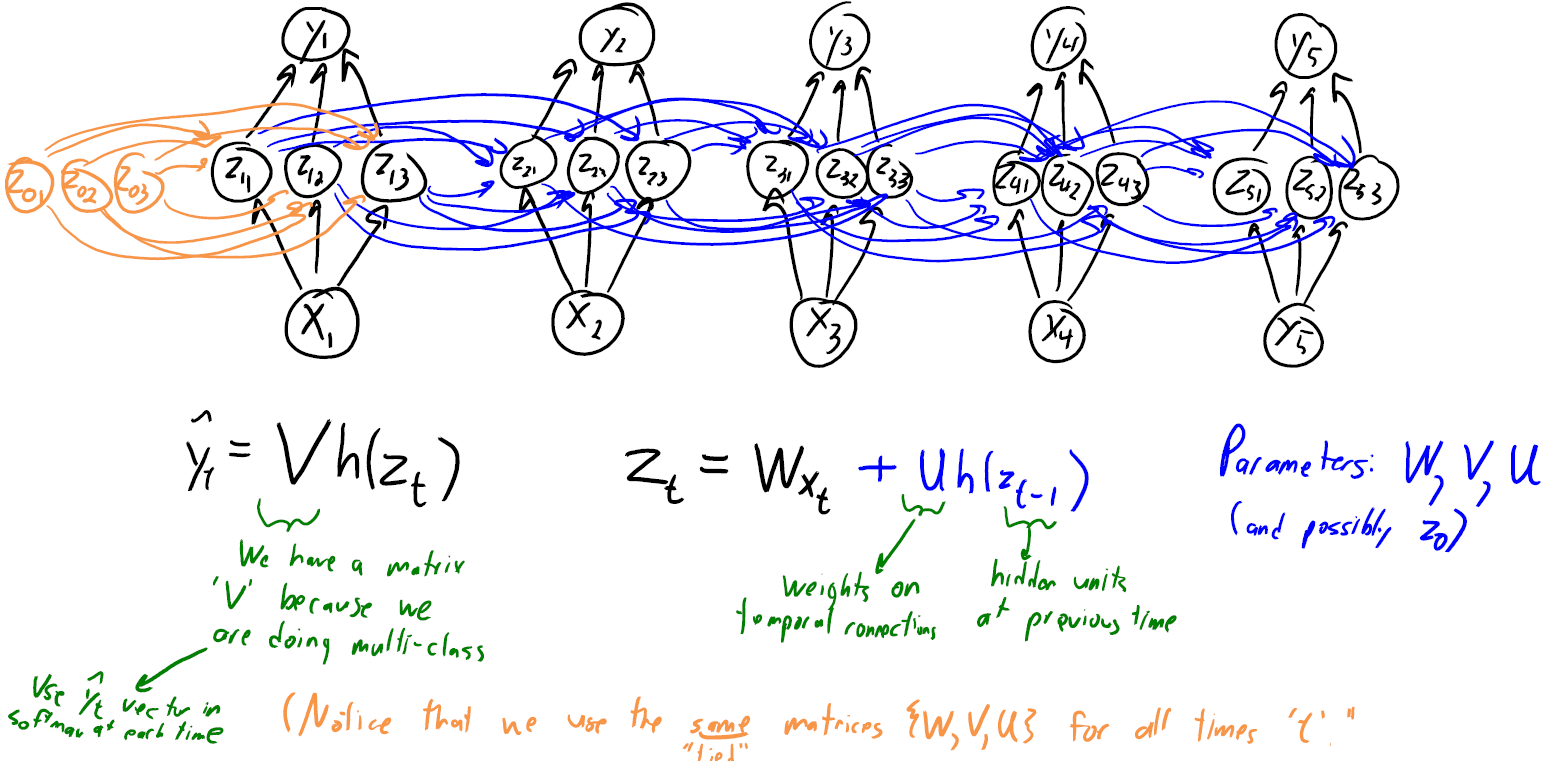
\includegraphics[width=\linewidth]{contents/rnn.png}
$k$ classes for each $\tilde{y}_t$, $m$ hidden units at each time, $T$ times\\
Total cost: $O(tmd+tkm+tk^2)$\\
Residual connections to transfer info forward in time more easily\\
Tied params to model sequences of diff length\\
\subsection*{RNN Issues}
vanishing/exploding grad\\
Consider $z^L=U^L z_0$, which diverges exponentially, or converges to zero.\\
Exponential Forgetting - use skip connections or memory\\
\subsection*{Sequence-to-Sequence RNNs}
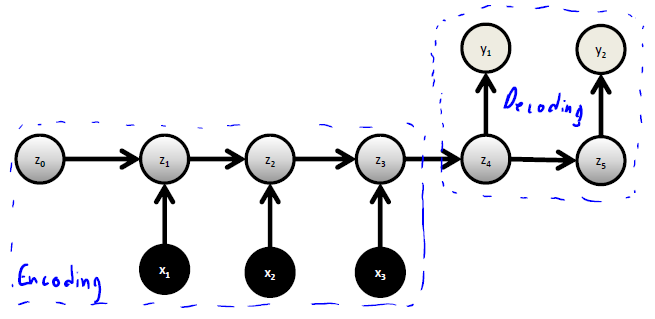
\includegraphics[width=\linewidth]{contents/s2s.png}
Sequence-to-sequence handles output sequences of unknown lengths - BOS at end of input, EOS at end of output.\\
Multi-modal learning considers input/output of diff formats
\subsection*{Long Short Term Memory (LSTM)}
Exponential Forgetting from standard RNNs\\
Memory cells with Gates\\
\[a_t=o_t\circ h_o(c_t)\in(-1,1)\]
\[c_t=f_t\circ c_{t-1} + i_t \circ g_t\in\mathbb{R}\]
\[o_t = h(W_o x_t + U_0 a_{t-1})\in(0,1)\]
\[f_t=h(W_f x_t+U_f a_{t-1})\in(0,1)\]
\[i_t=h(W_i x_t+U_i a_{t-1})\in(0,1)\]
\[g_t=h_o(W_g x_t+U_g a_{t-1})\in(-1,1)\]
\[\circ:\text{element-wise multiplication of vectors}\]
Usually gate function $h=$ sigmoid, value function $h_0=\tanh$.
Model longer-range dependencies than standard RNNs\\
Multi-Modal Learning - e.g. CNN as encoder and RNN as decoder for image-to-text
\subsection*{Attention and Transformers}
Problem w sequence-sequence RNN - all encoding info must be summarized by last state in encoder\\
Decoder access info from all encoding steps
\begin{itemize}
    \item Attention: Allow decoder to look at previous states
    \item Context Vectors: Combine previous states into a fixed-length vector, 
    as opposed to residual connections which requires same length inputs
    \item Dilated Convolutions for sequences ("with holes")
    \item Transformer Networks: \"Fully-connected\" attention, layers of \"self-attention\" to build context  
\end{itemize}
